\section{Methodology}

\subsection{Preliminary research}
To thoroughly understand the tool we are building, we will research various potentiometer designs. The lab work will be divided into the following areas: chemical, electrical, and software. Manufacturing and profiling the sensor will constitute the chemical component. Circuit simulation, circuit testing, and system design/implementation will constitute the hardware piece. Lastly, PC user interface and processing code will make up the software.

In order to contribute towards research, we plan to do a thorough literature review of existing glucose sensing techniques. This will include sensor manufacturing techniques and materials. Our design contribution will consist of schematics, system specification, and documentation of our design. We will also include data about profiling our glucose sensors.

\subsection{Sensor fabrication}
Sensor manufacturing process involves using lithography to create desired patterns of titanium on a silicon wafer. The wafer was prepared by depositing 3000 angstroms of SiO2 and then depositing 500 angstroms of Ti. After the metal is deposited, the wafer is slice into chucks of 2cm by 1cm. The sensor has 3 platinum electrodes: working, counter and, reference. The reference electrode is used to establish constant potential in electrochemical cell. The working electrode is where the electron transfer of interest occurs. Counter electrode is the one which completes the circuit. The working electrode forms a shape of a "lollipop" and contains the active area. A coat of photoresist is then applied to the wafer. The wafer is then exposed to UV with the first mask on top, developed, and then etched. A second layer of resist is applied and developed to help protect the wires and create the diamond pattern on the active area. Figure \ref{fig:stencils} shows the two stencils used for the masks during the UV exposure process. 

After a test strip is made, the strip has to be platinized and enzymes have to be deposited on the active area. Platinization is done by placing the wafer in hexachloroplatinic acid, connecting a platinum wire to the working electrode and applying a negative voltage to the wafer for a period of time. After platinization is done, the wafer is dried and is ready for enzyme immobilization. A receiving mixture of 2-Hydroxyethylmethacrylate (HEMA), Tetraethylenglycol diacrylate (TEGDA), and Polyethylenglycol methacrylate (PEGMA) is created to which a solution of glucose oxidase, ethylene glycol and DI water is added. A photo initiator, 2-dimethoxy- 2-phenylacetophenone (DMPA), is then added to the receiving mixture. This final mixture is deposited unto the active area of the wafer and the wafer is baked in a UV oven. 

\begin{figure} 
\begin{center}
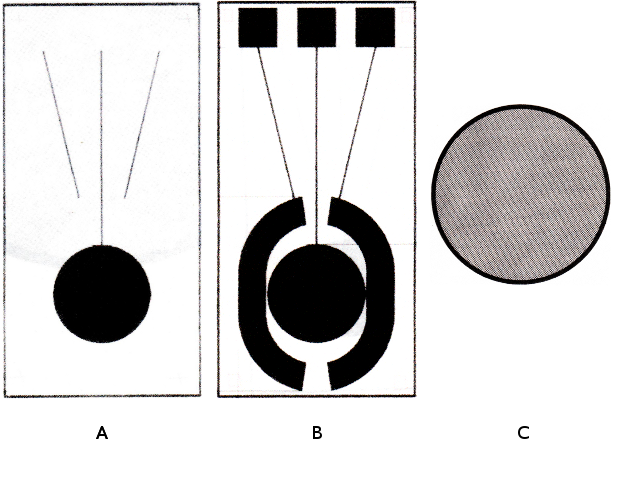
\includegraphics[width=3.5in]{../figures/stencils.png}
\end{center}
\caption{Stencils for lithography. {\bf A} is for the protective layer of resist. {\bf B} is the metal layer stencil. {\bf C} is a closeup of the diamond pattern on the active area.}
\label{fig:stencils}
\end{figure}


\subsection{Sensor characterization}
To characterize a sensor, it has to be subjected to a wide range of glucose concentrations and its current response recorder. We used commercial and custom made sensors with a commercial potentiostat in the amperometry mode. We tested three different concentrations: 1 mM, 5 mM and 10 mM.

\subsection{Potentiostat specification}
There are several characteristics that are desirable in this implementation. The device must be cheap, portable, and have a wide operating range. The system must also be able to transmit data to a PC where it can be visualized in real time. Before building the actual circuit, a simulation of the circuit has to be done to understand how the drive and measurement circuit works.


